% Тут используется класс, установленный на сервере Papeeria. На случай, если
% текст понадобится редактировать где-то в другом месте, рядом лежит файл matmex-diploma-custom.cls
% который в момент своего создания был идентичен классу, установленному на сервере.
% Для того, чтобы им воспользоваться, замените matmex-diploma на matmex-diploma-custom
% Если вы работаете исключительно в Papeeria то мы настоятельно рекомендуем пользоваться
% классом matmex-diploma, поскольку он будет автоматически обновляться по мере внесения корректив
%

% По умолчанию используется шрифт 14 размера. Если нужен 12-й шрифт, уберите опцию [14pt]
%\documentclass[14pt]{matmex-diploma}
\documentclass{matmex-diploma-custom}

\begin{document}
% Год, город, название университета и факультета предопределены,
% но можно и поменять.
% Если англоязычная титульная страница не нужна, то ее можно просто удалить.
\filltitle{ru}{
    chair              = {Кафедра небесной механики и звездной астрономии},
    title              = {Пространственно-кинематическое моделирование плоской подсистемы Галактики},
    % Здесь указывается тип работы. Возможные значения:
    %   coursework - Курсовая работа
    %   diploma - Диплом специалиста
    %   master - Диплом магистра
    %   bachelor - Диплом бакалавра
    type               = {diploma},
    position           = {студента},
    group              = 666,
    author             = {Волков Даниил Валентинович},
    supervisorPosition = {д.\,ф.-м.\,н., профессор},
    supervisor         = {Никифоров И.\,И.},
    reviewerPosition   = {ст. преп.},
    reviewer           = {Мосенков А.\,В.},
    chairHeadPosition  = {д.\,ф.-м.\,н., профессор},
    chairHead          = {Холшевников К.\,В.},
%   university         = {Санкт-Петербургский Государственный Университет},
    faculty            = {Математико-механический факультет},
%   city               = {Санкт-Петербург},
%   year               = {2013}
}
\filltitle{en}{
    chair              = {Chair of Celestial Mechanics},
    title              = {Modeling of the flat subsystem of the Galaxy},
    author             = {Daniil Volkov},
    supervisorPosition = {professor},
    supervisor         = {Igor Nikiforov},
    reviewerPosition   = {assistant},
    reviewer           = {Alexander Mosenkov},
    chairHeadPosition  = {professor},
    chairHead          = {Коnstantin Kholshevnikov},
}
\maketitle
\tableofcontents
% У введения нет номера главы
\section*{Введение}
Настоящая дипломная работа посвящена определению пространственных и кинематических параметров Галактики по её плоской подсистеме. То есть, это такие постоянные как расстояние до центра Галактики $R_0$ -- в данной работе центром Галактики будет считаться её барицентр, линейная скорость вращения Местного Стандарта Покоя (МСП) на солнечном круге $\Theta_0$, зависимость линейной скорости вращения от расстояния до оси вращения $\Theta(R)$. Выполняется построение кривых вращения. Также моделирование даёт и параметры солнечного движения относительно МСП ($u_{\odot}, v_{\odot}, w_{\odot}$).
\par Несмотря на то, что проблеме определения $R_0$ уже очень много лет (первые оценки были сделаны Shapley в 1918 году), усовершенствование имеющихся и разработка новых методов определения $R_0$ является актуальной задачей и по сей день. Относительно недавно, в 2004 году, Пачиньский и Станек выдвинули \texttt{звезды красного сгущения} как новый индикатор расстояний и использовали эти звезды как опорные объекты для опредления $R_0$ методом Бааде.
\par Звезды красного сгущения -- это высокометалличный аналог горизонтальной ветви, состоящий из населения II типа. Преимущество этих звезд как опорных объектов -- в их многочисленности, что дает высокую статистическую точность оценки $R_0$. Также Станек и др. (2000) показали, что средняя абсолютная звездная величина ЗКС слабо меняется с возрастом и металличностью. В настоящей работе к этим опорным объектам применяется трехкомпонентная кинематическая модель. Также полностью определено воспроизведение конечной выборки, по которой получается решение. Кроме того, в отличии от многих подобных работ в этой области, здесь оптимизируется и порядок модели (модельных полиномов), а также применяется гибкий алгоритм исключения из выборки объектов с большими невязками.

\section{Пространственно-кинематическое моделирование плоской подсистемы}

\subsection{Основные предположения и определения}
\textbf{Предположение 1.}
Зависимость линейной скорости $\Theta$ движения подсистем Галактики -- это функция галактоосевого расстояния $R$: 
\begin{equation}
        \Theta = \Theta(R).
\end{equation}

\textbf{Предположение 2.}
Предполагается нормальное распределение ошибок, так как в данной работе применяется метод наименьших квадратов.

\textit{Модельная скорость} заданного объекта -- скорость центроида объектов данного типа, вычисленная для положения этого объекта.

\textit{Вращательный стандарт покоя} (ВСП) -- гелиоцентрическая система отсчета, движущаяся по круговой орбите со скоростью равной средней скорости вращения рассматриваемой подсистемы на $R = R_0$.

Вклад в модельную скорость вращения подсистемы -- $V_{\texttt{rot}}$.

Вклад в модельную скорость движения Солнца относительно ВСП подсистемы -- $V_{\odot}$.

Компоненты скорости движения Солнца относительно ВСП: $u_{\odot}, v_{\odot}, w_{\odot}$.


\subsection{Математическая модель}
Для представления $\Theta(R)$ используем модельный полином в виде многочлена Тейлора:
\begin{equation} \label{theta_n}
        \Theta_n(R)=\sum _{i=0}^{n} \frac{d^i\Theta \cdot (R - R_0)^i}{dR^i\cdot i!}.
\end{equation}
\begin{equation}
	R = \sqrt{R_0^2 + r^2 \cos^2{b} - 2R_0 r \cos{l} \cos{b}}.
\end{equation}

Здесь и далее $l$ -- галактическая долгота, $b$ -- галактическая широта, $r$ -- гелиоцентрическое расстояние.
\pagebreak
\subsubsection{Лучевые скорости} \label{def_mod_vr}
\begin{equation}
        V_{r, \texttt{rot}} = (\omega - \omega_0)R_0 \sin{l} \cos{b},
\end{equation}
\begin{equation}
        V_{r, \odot} = -u_{\odot} \cos{l} \cos{b} - v_{\odot} \cos{b} \sin{l} - w_{\odot} \sin{b}.
\end{equation}

\begin{equation}
        V_{r, \texttt{mod}} = \left[ -2A\Delta R + \sum^n_{k = 2} \frac{\theta_k}{k!} \left( \Delta R \right)^k \right] \frac{R_0}{R} \sin{l} \cos{b} + V_{r, \odot},
\end{equation}
\begin{equation}
        A = - \frac{1}{2} R_0 \omega^{'}(R_0) = - \frac{1}{2} (\theta_1 - \omega_0).
\end{equation}
\subsubsection{Собственные движения по широте} \label{def_mod_b}
Для собственных движений $\mu_b = \frac{db}{dt}$:
\begin{equation}
        k\mu_{b, \texttt{mod}} = k\mu_{b, \texttt{rot}} + k\mu_{b, \odot},
\end{equation}
\begin{equation}
        k\mu_{b, \texttt{rot}} = \left[ 2A\Delta R - \sum^n_{k = 2} \frac{\theta_k}{k!} \left( \Delta R \right)^k \right] \frac{R_0}{Rr} \sin{l} \sin{b},
\end{equation}
\begin{equation}
        k\mu_{b, \odot} = \frac{u_{\odot}\cos{l}\sin{b} + v_{\odot}\sin{l}\sin{b} - w_{\odot}\cos{b}}{r}.
\end{equation}
Здесь и далее полагаем $k=4.7406$.
\subsubsection{Собственные движения по долготе} \label{def_mod_l}
Для собственных движений $\mu_l = \frac{dl}{dt}\cos{b}$:
\begin{equation}
        k\mu_{l, \texttt{mod}} = k\mu_{l, \texttt{rot}} + k\mu_{l, \odot},
\end{equation}
\begin{equation}
        k\mu_{l, \texttt{rot}} = \left[ -2A\Delta R + \sum^n_{k = 2} \frac{\theta_k}{k!} \left( \Delta R \right)^k \right] \left( \frac{R_0\cos{l}}{r} - \cos{b} \right) R^{-1} - \omega_0 \cos{b},
\end{equation}
\begin{equation}
        k\mu_{b, \odot} = \frac{u_{\odot}\sin{l}- v_{\odot}\cos{l}}{r}.
\end{equation}



\subsubsection{Общее решение}
Имеется набор систем уравнений
\begin{equation} \label{v_r_sys}
                V_r = V_{r, \texttt{mod}} (R_0, A, \theta_2, \:\ldots,\: \theta_n, u_{\odot}, v_{\odot}, w_{\odot}^{*}),
	\end{equation}
        \begin{equation} \label{b_sys}
                k\mu_b = k\mu_{b, \texttt{mod}} (R_0^{*}, A, \theta_2, \:\ldots,\: \theta_n, u_{\odot}, v_{\odot}, w_{\odot}^{*}).
	\end{equation}
        \begin{equation} \label{l_sys}
                k\mu_l = k\mu_{l, \texttt{mod}} (R_0^{*}, A, \theta_2, \:\ldots,\: \theta_n, u_{\odot}, v_{\odot}),
	\end{equation}
        Здесь индекс опущен, $V_r, k\mu_l, k\mu_b$ -- наблюдаемые величины. Параметры со звездочкой \textit{могут} фиксироваться. Модельные скорости определены согласно \ref{def_mod_vr}, \ref{def_mod_b}, \ref{def_mod_l}. Каждая из этих систем решается обычным МНК с единичными весами. Частное решение (при фиксированном единственном нелинейном параметре $R_0$) можно найти стандарным линейным МНК. Тогда общее решение дает значение $R_0$, при котором целевая функция минимальна. 
\par Найденные общие решения дают оценки дисперсий:
	\begin{equation}
                \sigma^2_{V_r} = \frac{1}{N_{\texttt{free}}} \sum^N_{i = 1} \left( V_r - V_{r, \texttt{mod}} \right)^2_i,
	\end{equation}
	\begin{equation}
                \sigma^2_{\mu_l} = \frac{1}{N_{\texttt{free}}} \sum^N_{i = 1} \left( k\mu_l - k\mu_{l, \texttt{mod}} \right)^2_i,
	\end{equation}
	\begin{equation}
                \sigma^2_{\mu_b} = \frac{1}{N_{\texttt{free}}} \sum^N_{i = 1} \left( k\mu_b - k\mu_{b, \texttt{mod}} \right)^2_i,
	\end{equation}
        где число степеней свободы $N_{\texttt{free}} = N - n_{\texttt{par}}$.

При фиксации линейных параметров решение систем итеративное. 

Итерация 1:
\begin{enumerate}
        \item Решается (\ref{v_r_sys}) с начальным значением $w_{\odot} = \textrm{const}$. Получаем оценку $R_0(V_r)$.
        \item Решается (\ref{b_sys}) при $R_0 = const = R_0(V_r)$. Получаем оценку $w_{\odot}(\mu_b)$.
\end{enumerate}
\par Итерация I:
\begin{enumerate}
        \item Решается (\ref{v_r_sys}) при $w_{\odot} = const = w_{\odot}(\mu_b)_{I - 1}$. Получаем оценку $R_0(V_r)_I$.
        \item Решается (\ref{b_sys}) при $R_0 = const = R_0(V_r)_I$. Получаем оценку $w_{\odot}(\mu_b)_I$.
\end{enumerate}
Условие сходимости -- неизменность $m$ десятичных знаков после запятой в значениях обоих параметров. После достижения условия сходимости за $T$ итераций решается система (\ref{l_sys}) с $R_0^{*}=R_0(V_r)_{I_T}$.

Далее минимизируется целевая функция

\begin{equation} \label{chi_sq_func}
                \chi^2 = \sum^N_{i = 1} \left[ \frac{\left( V_r - V_{r, \texttt{mod}} \right)^2_i}{\sigma^2_{V_r}} + \frac{\left( \mu_l - \mu_{l, \texttt{mod}} \right)^2_i}{\sigma^2_{\mu_l}} + \frac{\left( \mu_b - \mu_{b, \texttt{mod}} \right)^2_i}{\sigma^2_{\mu_b}} \right].
	\end{equation}
Используются значения $\sigma^2_{V_r}, \sigma^2_{\mu_b}, \sigma^2_{\mu_l}$, найденные после итеративного решения систем (\ref{v_r_sys}) - (\ref{l_sys}). Значение $\chi^2$ должно быть около $N_{\texttt{free}} = 3 N - n_{par}$. 

\pagebreak
\subsection{Построение кривых вращения}
\subsubsection{Решение по лучевым скоростям}
Кривая вращения:
\begin{equation}
        \Theta_n(R) = \omega_0 R - 2A\Delta R + \sum^n_{k = 2} \frac{\theta_k}{k!} \left( \Delta R \right)^k ,
\end{equation}

Положения отдельных объектов (здесь $V_{\texttt{obs}}$ -- наблюдаемая величина):
\begin{equation}
        \Theta_{\texttt{obs}}(R) = \left( \frac{V_{\texttt{obs}} - V_{r, \odot}}{R_0 \sin{l} \cos{b}} + \omega_0 \right) R.
\end{equation}
\subsubsection{Решение по собственным широтным движениям}
Кривая вращения:
\begin{equation}
        \Theta_n(R) = \omega_0 R + 2A\Delta R - \sum^n_{k = 2} \frac{\theta_k}{k!} \left( \Delta R \right)^k ,
\end{equation}

Положения отдельных объектов (здесь $\mu_{b, \texttt{obs}}$ -- наблюдаемая величина):
\begin{equation}
        \Theta_{\texttt{obs}}(R) = \left( \frac{k\mu_{b, \odot} - k\mu_{b, \texttt{obs}}}{R_0 \sin{l} \sin{b}} r + \omega_0 \right) R.
\end{equation}
\subsubsection{Решение по собственным долготным движениям}
Кривая вращения:
\begin{equation}
        \Theta_n(R) = \omega_0 R - 2A\Delta R + \sum^n_{k = 2} \frac{\theta_k}{k!} \left( \Delta R \right)^k ,
\end{equation}

Положения отдельных объектов (здесь $\mu_{l, \texttt{obs}}$ -- наблюдаемая величина):
\begin{equation}
        \Theta_{\texttt{obs}}(R) = \left( \frac{k\mu_{l, \texttt{obs}} - k\mu_{l, \odot} + \omega_0 \cos{b}}{\frac{R_0 \cos{l}}{r} - \cos{b}} r + \omega_0 \right) R.
\end{equation}




\section{Формирование выборки}
\subsection{Исключение объектов по избыточным невязкам} \label{err_filter}
Для многих процедур статистического анализа наблюдательного материала важной проблемой является обоснованное выделение и исключение из обработки ненадежных данных. Так как используемый объем выборки довольно велик, то объектов, которые имеют невязки больше $3\sigma$, может быть довольно много. В источнике (N) предложен следующий гибкий алгоритм исключения объектов из выборки, который и используется в данной работе:

\par Для данного объема выборки $N$ находится значение $\kappa$:
\begin{equation}
\psi (\kappa) = \sqrt{\frac{2}{\pi}} \int_0^{\kappa} e^{- \frac{x^2}{2}} dx,
\end{equation}
\begin{equation}
\left[ 1 - \psi (\kappa) \right] N = 1.
\end{equation}
Тогда, обозначая $\epsilon_i$ - ошибку $i$-того измерения, а $\sigma_i$ - стандартная ошибка $i$-того измерения, получаем критерий
\begin{equation} \label{criteria}
\frac{\left| \epsilon_i \right|}{\sigma_i} > \kappa.
\end{equation}
Далее находится количество уравнений $L$ данной выборки, которые удовлетворяют этому условию. Если $L > 1$, то из дальнейшего рассмотрения исключается $L - L_p$ уравнений с наибольшими по модулю невязками, где $L_p$ — параметр данного алгоритма.  В настоящей работе $L_p = 1$.

\subsection{Исключение пространственно изолированных объектов}
Так как объекты, удаленные от основной массы выборки, способны сильно влиять на результат, предлагается такие объекты также исключать из выборки. В ранных релизах каталога опорных объектов, которые были использованы в даннной работе, такие объекты имелись. Однако в последнем релизе были улучшены редукции за поглощение, и явных выбросов по пространственному распределению объектов не наблюдается (см. далее [ссылка на диаграмму]).

\section{Оптимизация модели}
\subsection{Оптимизация порядка модельных полиномов}
Итак, $\Theta_n(R)$ есть полином Тейлора(\ref{theta_n}) степени $n$. В большинстве работ (ссылки) $n$ не превосходит 2. Здесь мы можем исследовать и более высокие порядки, так как объем выборки позволяет нам выявлять более мелкие детали на кривой вращения (например, её прогиб после солнечного круга, в работах (ссылки)). Для того, чтобы определить оптимальный порядок разложения, будем руководствоваться следующими критериями.
Порядок разложения ограничен сверху таким $n$, что
\begin{enumerate}
        \item Все коэффициенты $\theta_i$ становятся незначимыми: $\frac{\theta_i}{\sigma_{\theta_i}}\approx 0.5$, \label{crit_1}
        \item Значимость коэффициента $\theta_n$ снижается до $1 \sigma$,  \label{crit_2}
        \item Значение дисперсии решения перестаёт значимо убывать, \label{crit_3}
        \item На кривой вращения отчетливо проявляются краевые эффекты. \label{crit_4}
\end{enumerate}

Выбор того, какой из критериев в данном случае применим, пока не формализован полностью. В большинстве случаев срабатывает критерий \ref{crit_2}. В данной работе были предприняты попытки использования каких-либо мер для оптимизации порядка (например, мера Меллоуза (ссылка)), но добиться полной формализации с сохранением всех указанных условий не удалось.

\subsection{Оптимизация оценки $R_0$}
В уравнениях (\ref{v_r_sys}) -- (\ref{l_sys}), а также в (\ref{chi_sq_func}) параметр $R_0$ нелинейный. Поэтому для поиска решения таких систем уравнений мы рассматриваем частные решения при фиксированном $R_0$ и минимизируем целевую функцию. Для систем (\ref{v_r_sys}) -- (\ref{l_sys}) целевая функция есть
\begin{equation}
        \chi^2 = \sum_{i=1}^{N} \left [ V_{i, \texttt{mod}} - V_{i, \texttt{obs}} \right ]^2.
\end{equation}
Зависимость $\chi^2(R_0)$ в дальнейшем будет называться \textit{профилем решения}.

\section{Применение метода к данным о звездах красного сгущения}
\subsection{Данные об опорных объектах}
Сведения, необходимые для моделирования, брались из каталога APOGEE-RC (Data Release 14, на ранних этапах работы также использовались DR 13 и 12)[ref], полученного по результатам SDSS[ref]. Из всего набора параметров использовались следующие: 
\begin{table}[ht]
\centering
\caption{Наблюдательные данные (приведены на эпоху \texttt{J2000})}
\begin{tabular}{|l|l|l|l|}
\hline
\textbf{Поле} & \textbf{Значение} & \textbf{Обозначение} & \textbf{Ед. изм.} \\
\hline
\texttt{RA} & Прямое восхождение & $\alpha$ & deg \\
\texttt{DEC} & Склонение & $\delta$ & deg \\
\texttt{GLON} & Галактическая долгота & $l$ & deg \\
\texttt{GLAT} & Галактическая широта & $b$ & deg \\
\hline
\texttt{VHELIO\_AVG} & Гелиоцентрическая скорость & $V_{r, \texttt{obs}}$ & km/s \\
\texttt{RC\_DIST} & Гелиоцентрическое расстояние & $r$ & kpc \\
\hline
\texttt{PMRA} & Проекция собственного движения по $\alpha$  & $\mu_{\alpha}* \cos{\delta}$ & mas/yr \\
\texttt{PMDEC} & Собственное движение по $\delta$  & $\mu_{\delta}$ & mas/yr \\
\texttt{PMRA\_ERR} & Ошибка собственного движения по $\alpha$  & $\sigma_{\mu_{\alpha}, i}$ & mas/yr \\
\texttt{PMDEC\_ERR} & Ошибка собственного движения по $\delta$  & $\sigma_{\mu_{\delta}, i}$ & mas/yr \\
\texttt{PMMATCH} & Индикатор отождествления объекта  & -- & -- \\
\hline
\texttt{PMRA\_HSOY} & Проекция собственного движения по $\alpha$  & $\mu_{\alpha}* \cos{\delta}$ & mas/yr \\
\texttt{PMDEC\_HSOY} & Собственное движение по $\delta$  & $\mu_{\delta}$ & mas/yr \\
\texttt{PMRA\_ERR\_HSOY} & Ошибка собственного движения по $\alpha$  & $\sigma_{\mu_{\alpha}, i}$ & mas/yr \\
\texttt{PMDEC\_ERR\_HSOY} & Ошибка собственного движения по $\delta$  & $\sigma_{\mu_{\delta}, i}$ & mas/yr \\
\texttt{PMMATCH\_HSOY} & Индикатор отождествления объекта  & -- & -- \\
\hline
\end{tabular}
\end{table}

\pagebreak
\subsubsection{Дополнительные преобразования данных}
Так как в каталогах \texttt{UCAC-4} и \texttt{HSOY} указаны данные о собственных движениях в экваториальной СК, нужно было осуществить преобразование $(\mu_{\alpha}, \mu_{\delta}) \rightarrow (\mu_l, \mu_b)$.
\begin{equation}
        \sin{b} = \sin{\delta} \cos(90^{\circ} - \delta_p) - \cos{\delta} \sin(\alpha - \alpha_p - 90^{\circ}) \sin(90^{\circ} - \delta_p),
\end{equation}
\begin{equation}
        \sin{\varphi} = \frac{\cos{\delta} \sin(\alpha - \alpha_p - 90^{\circ}) \cos(90^{\circ} - \delta_p) + \sin{\delta} \sin(90^{\circ} - \delta_p)}{\cos{b}},
\end{equation}
\begin{equation}
        \cos{\varphi} = \frac{ \cos{\delta} \cos(\alpha - \alpha_p - 90^{\circ})}{\cos{b}},
\end{equation}
\begin{equation}
        l = \varphi + \theta_p,
\end{equation}
где $\theta_p = 32.93192^{\circ}$, $\alpha_p = 192.85948^{\circ}$, $\delta_p = 27.12825^{\circ}$. Переход к собственным движениям в галактической СК:
\begin{equation}
        \mu_l = l(\alpha + \mu_{\alpha}, \delta + \mu_{\delta}) - l(\alpha, \delta),
\end{equation}
\begin{equation}
        \mu_b = b(\alpha + \mu_{\alpha}, \delta + \mu_{\delta}) - b(\alpha, \delta).
\end{equation}
Также необходимо подставлять в (\ref{l_sys}) $\mu_l^* = \mu_l \cos{b}$.

\subsubsection{Формирование выборок для оценки ошибок параметров методом Монте-Карло} \label{mk}
Несмотря на то, что при частном решении используется обычный МНК, получать из матрицы ковариаций ошибки параметров некорректно, так как производится оптимизация по нелинейному параметру. Для того, чтобы исключить смещение и обеспечить состоятельность и эффектривность оценки ошибков параметров модели, используется метод Монте-Карлою. Для получения ошибок параметров при решении (\ref{v_r_sys}) - (\ref{l_sys}), а также (\ref{chi_sq_func}), формируются псевдослучайные каталоги. В каждом из них такие же сведения о $l$, $b$, $r$, \texttt{PMMATCH}, как в оригинальном \texttt{APOGEE-RC} ($\alpha$ и $\delta$ для решения систем не нужны). Лучевые скорости и собственные движения получались как
\begin{equation}
        V_{r, i}^{*} \in \mathcal{N} \left[ V_{r, \texttt{mod}}(l_i, b_i, r_i),\sigma_{V_r} \right],
\end{equation}
\begin{equation}
        \mu_{b, i}^{*} \in \mathcal{N} \left[ \mu_{b, \texttt{mod}}(l_i, b_i, r_i),\sigma_{\mu_b} \right],
\end{equation}
\begin{equation}
        \mu_{l, i}^{*} \in \mathcal{N} \left[ \mu_{l, \texttt{mod}}(l_i, b_i, r_i),\sigma_{\mu_l} \right].
\end{equation}
\par После этого для каждого каталога находятся все параметры модели и строится кривая вращения. По совокупности всех найденных значений производится окончательная оценка параметров и построение доверительных областей кривой вращения.
\pagebreak
\subsection{Моделирование по лучевым скоростям}
Решается (\ref{v_r_sys}) с полным набором параметров. Порядок разложения $n < 10$. Итеративно применяется \ref{err_filter}, пока в выборке не будет объектов, попадающих под критерий (\ref{criteria}). После этого производится оценка ошибок параметров с помощью \ref{mk} по финальной выборке размера $N_{\texttt{end}}$. Результаты приведены в таблице. 
\begin{table}[h!!]
\centering
\caption{Результаты.}
\begin{tabular}{r|rrrrrrrrrr}
\hline
$n$ & $1$ & $2$ & $3$ & $\textbf{4}$ & $5$&$ 6 $&$ 7 $&$ 8 $&$ 9 $&$ 10 $\\\hline
$N_{\texttt{end}}$ & $1$ & $2$ & $3$ & $\textbf{4}$ & $5$&$ 6 $&$ 7 $&$ 8 $&$ 9 $&$ 10 $\\\hline
 $R_0 $&$     8.73$&$    8.73$&$    8.20$&$   \textbf{ 8.25}$&$    8.20$&$    8.18$&$    8.26$&$    8.27$&$    8.37$&$    8.54$\\$
 \sigma_{R_0} $&$     0.26$&$    0.32$&$   0.26$&$  \textbf{  0.25}$&$    0.25$&$    0.26$&$    0.28$&$    0.28$&$    0.30$&$    0.31$\\$
 \sigma_{V_r} $&$    30.50$&$   30.50$&$   30.36$&$  \textbf{ 30.36}$&$   30.35$&$   30.35$&$   30.35$&$   30.35$&$   30.34$&$   30.33$\\\hline$
 u_{\odot} $&$    13.19$&$   13.19$&$   13.56$&$  \textbf{ 13.61}$&$   13.61$&$   13.62$&$   13.60$&$   13.60$&$   13.58$&$   13.57$\\$
 \sigma_{u_{\odot}} $&$     0.30$&$    0.31$&$    0.31$&$   \textbf{ 0.31}$&$    0.31$&$    0.31$&$    0.31$&$    0.31$&$    0.31$&$    0.31$\\\hline$
 v_{\odot} $&$    27.12$&$   27.11$&$   24.92$&$  \textbf{ 25.41}$&$   25.00$&$   25.02$&$   24.77$&$   24.69$&$   24.25$&$   24.45$\\$
 \sigma_{v_{\odot}}$&$     0.41$&$    0.45$&$    0.46$&$   \textbf{ 0.48}$&$    0.50$&$    0.51$&$    0.53$&$    0.53$&$    0.56$&$    0.56$\\\hline$
 w_{\odot} $&$     3.96$&$    3.96$&$    4.70$&$   \textbf{ 4.71}$&$    4.85$&$    4.86$&$    4.93$&$    4.88$&$    4.97$&$    5.00$\\$
 \sigma_{w_{\odot}} $&$     0.84$&$    0.84$&$    0.84$&$   \textbf{ 0.84}$&$    0.84$&$    0.84$&$    0.84$&$    0.84$&$    0.84$&$    0.84$\\\hline$
 A $&$    13.44$&$   13.44$&$   15.35$&$  \textbf{ 15.85}$&$   16.05$&$   16.15$&$   16.23$&$   15.77$&$   15.66$&$   16.08$\\$
 \sigma(A) $&$     0.13$&$    0.15$&$    0.20$&$   \textbf{ 0.25}$&$    0.26$&$    0.31$&$    0.32$&$    0.39$&$    0.39$&$    0.45$\\$
 \theta_2$&$ $-$ $&$   -0.00$&$   -1.64$&$   \textbf{-0.62}$&$   -1.49$&$   -1.37$&$   -2.61$&$   -2.94$&$   -5.66$&$   -5.80$\\$
 \sigma(\theta_2)$&$ $-$ $&$    0.18$&$    0.21$&$  \textbf{  0.35}$&$    0.50$&$    0.56$&$    0.79$&$    0.81$&$    1.13$&$    1.13$\\$
 \theta_3$&$ $-$ $&$ $-$ $&$    2.35$&$   \textbf{ 3.03}$&$    3.77$&$    4.04$&$    4.87$&$    2.54$&$    2.78$&$    6.41$\\$
 \sigma(\theta_3)$&$ $-$ $&$ $-$ $&$    0.18$&$   \textbf{ 0.26}$&$    0.40$&$    0.66$&$    0.77$&$    1.37$&$    1.37$&$    2.16$\\$
 \theta_4$&$ $-$ $&$ $-$ $&$ $-$ $&$  \textbf{ -0.78}$&$   -0.10$&$   -0.33$&$    1.71$&$    3.06$&$   10.59$&$   10.43$\\$
 \sigma(\theta_4)$&$ $-$ $&$ $-$ $&$ $-$ $&$   \textbf{ 0.22}$&$    0.36$&$    0.58$&$    1.06$&$    1.24$&$    2.48$&$    2.51$\\$
 \theta_5$&$ $-$ $&$ $-$ $&$ $-$ $&$ $-$ $&$   -0.70$&$   -0.92$&$   -2.64$&$    1.21$&$   -1.79$&$  -12.10$\\$
 \sigma(\theta_5)$&$ $-$ $&$ $-$ $&$ $-$ $&$ $-$ $&$    0.29$&$    0.52$&$    0.93$&$    2.09$&$    2.27$&$    5.07$\\$
 \theta_6$&$ $-$ $&$ $-$ $&$ $-$ $&$ $-$ $&$ $-$ $&$    0.23$&$   -1.48$&$   -4.59$&$  -18.41$&$  -14.87$\\$
 \sigma(\theta_6)$&$ $-$ $&$ $-$ $&$ $-$ $&$ $-$ $&$ $-$ $&$    0.45$&$    0.86$&$    1.74$&$    4.31$&$    4.72$\\$
 \theta_7$&$ $-$ $&$ $-$ $&$ $-$ $&$ $-$ $&$ $-$ $&$ $-$ $&$    1.80$&$   -1.49$&$    8.18$&$   28.37$\\$
 \sigma(\theta_7)$&$ $-$ $&$ $-$ $&$ $-$ $&$ $-$ $&$ $-$ $&$ $-$ $&$    0.79$&$    1.79$&$    3.30$&$    9.36$\\$
 \theta_8$&$ $-$ $&$ $-$ $&$ $-$ $&$ $-$ $&$ $-$ $&$ $-$ $&$ $-$ $&$    3.46$&$   16.45$&$    3.05$\\$
 \sigma(\theta_8)$&$ $-$ $&$ $-$ $&$ $-$ $&$ $-$ $&$ $-$ $&$ $-$ $&$ $-$ $&$    1.69$&$    4.09$&$    7.38$\\$
 \theta_9$&$ $-$ $&$ $-$ $&$ $-$ $&$ $-$ $&$ $-$ $&$ $-$ $&$ $-$ $&$ $-$ $&$  -12.98$&$  -33.60$\\$
 \sigma(\theta_9)$&$ $-$ $&$ $-$ $&$ $-$ $&$ $-$ $&$ $-$ $&$ $-$ $&$ $-$ $&$ $-$ $&$    3.73$&$    9.64$\\$
 \theta_{10}$&$ $-$ $&$ $-$ $&$ $-$ $&$ $-$ $&$ $-$ $&$ $-$ $&$ $-$ $&$ $-$ $&$ $-$ $&$   20.41$\\$
 \sigma(\theta_{10})$&$ $-$ $&$ $-$ $&$ $-$ $&$ $-$ $&$ $-$ $&$ $-$ $&$ $-$ $&$ $-$ $&$ $-$ $&$    8.94$\\
\end{tabular}
\end{table}

\pagebreak
\paragraph{Кривая вращения.} Приводятся кривые вращения, полученные для различных $n$. При построении полагали значение $\omega_{\odot} = 30.5$ км/c/кпк.
\begin{figure}[h!]
\begin{minipage}[h]{0.49\linewidth}
        \includegraphics[width=0.9\textwidth]{../result_1_100_apogee-ucac_vr/apogee-ucac.txt_1.eps}
\end{minipage}
\hfill
\begin{minipage}[h]{0.49\linewidth}
        \includegraphics[width=0.9\textwidth]{../result_2_100_apogee-ucac_vr/apogee-ucac.txt_2.eps}
\end{minipage}
\end{figure}
\begin{figure}[h!]
\begin{minipage}[h]{0.49\linewidth}
        \includegraphics[width=0.9\textwidth]{../result_3_100_apogee-ucac_vr/apogee-ucac.txt_3.eps}
\end{minipage}
\hfill
\begin{minipage}[h]{0.49\linewidth}
        \includegraphics[width=0.9\textwidth]{../result_4_100_apogee-ucac_vr/apogee-ucac.txt_4.eps}
\end{minipage}
\end{figure}
\begin{figure}[h!]
\begin{minipage}[h]{0.49\linewidth}
        \includegraphics[width=0.9\textwidth]{../result_5_100_apogee-ucac_vr/apogee-ucac.txt_5.eps}
\end{minipage}
\hfill
\begin{minipage}[h]{0.49\linewidth}
        \includegraphics[width=0.9\textwidth]{../result_6_100_apogee-ucac_vr/apogee-ucac.txt_6.eps}
\end{minipage}
\end{figure}


\pagebreak
\subsection{Моделирование по собственным широтным движениям}
Решается (\ref{b_sys}) с полным набором параметров. Порядок разложения $n < 10$. Итеративно применяется \ref{err_filter}, пока в выборке не будет объектов, попадающих под критерий (\ref{criteria}). После этого производится оценка ошибок параметров с помощью \ref{mk} по финальной выборке размера $N_{\texttt{end}}$. Результаты приведены в таблице. 
\begin{table}[h!!]
\centering
\caption{Результаты.}
\begin{tabular}{r|rrrrrrrrrr}
\hline
$n$ & $1$ & $2$ & $3$ & $\textbf{4}$ & $5$&$ 6 $&$ 7 $&$ 8 $&$ 9 $&$ 10 $\\\hline
$N_{\texttt{end}}$ & $1$ & $2$ & $3$ & $\textbf{4}$ & $5$&$ 6 $&$ 7 $&$ 8 $&$ 9 $&$ 10 $\\\hline
 $ R_0 $&$     8.73$&$    8.73$&$    8.20$&$   \textbf{ 8.25}$&$    8.20$&$    8.18$&$    8.26$&$    8.27$&$    8.37$&$    8.54$\\$
 \sigma_{R_0} $&$     0.26$&$    0.32$&$   0.26$&$  \textbf{  0.25}$&$    0.25$&$    0.26$&$    0.28$&$    0.28$&$    0.30$&$    0.31$\\$
 \sigma_{\mu_b} $&$    30.50$&$   30.50$&$   30.36$&$  \textbf{ 30.36}$&$   30.35$&$   30.35$&$   30.35$&$   30.35$&$   30.34$&$   30.33$\\\hline$
 u_{\odot} $&$    13.19$&$   13.19$&$   13.56$&$  \textbf{ 13.61}$&$   13.61$&$   13.62$&$   13.60$&$   13.60$&$   13.58$&$   13.57$\\$
 \sigma_{u_{\odot}} $&$     0.30$&$    0.31$&$    0.31$&$   \textbf{ 0.31}$&$    0.31$&$    0.31$&$    0.31$&$    0.31$&$    0.31$&$    0.31$\\\hline$
 v_{\odot} $&$    27.12$&$   27.11$&$   24.92$&$  \textbf{ 25.41}$&$   25.00$&$   25.02$&$   24.77$&$   24.69$&$   24.25$&$   24.45$\\$
 \sigma_{v_{\odot}}$&$     0.41$&$    0.45$&$    0.46$&$   \textbf{ 0.48}$&$    0.50$&$    0.51$&$    0.53$&$    0.53$&$    0.56$&$    0.56$\\\hline$
 w_{\odot} $&$     3.96$&$    3.96$&$    4.70$&$   \textbf{ 4.71}$&$    4.85$&$    4.86$&$    4.93$&$    4.88$&$    4.97$&$    5.00$\\$
 \sigma_{w_{\odot}} $&$     0.84$&$    0.84$&$    0.84$&$   \textbf{ 0.84}$&$    0.84$&$    0.84$&$    0.84$&$    0.84$&$    0.84$&$    0.84$\\\hline$
 A $&$    13.44$&$   13.44$&$   15.35$&$  \textbf{ 15.85}$&$   16.05$&$   16.15$&$   16.23$&$   15.77$&$   15.66$&$   16.08$\\$
 \sigma(A) $&$     0.13$&$    0.15$&$    0.20$&$   \textbf{ 0.25}$&$    0.26$&$    0.31$&$    0.32$&$    0.39$&$    0.39$&$    0.45$\\$
 \theta_2$&$ $-$ $&$   -0.00$&$   -1.64$&$   \textbf{-0.62}$&$   -1.49$&$   -1.37$&$   -2.61$&$   -2.94$&$   -5.66$&$   -5.80$\\$
 \sigma(\theta_2)$&$ $-$ $&$    0.18$&$    0.21$&$  \textbf{  0.35}$&$    0.50$&$    0.56$&$    0.79$&$    0.81$&$    1.13$&$    1.13$\\$
 \theta_3$&$ $-$ $&$ $-$ $&$    2.35$&$   \textbf{ 3.03}$&$    3.77$&$    4.04$&$    4.87$&$    2.54$&$    2.78$&$    6.41$\\$
 \sigma(\theta_3)$&$ $-$ $&$ $-$ $&$    0.18$&$   \textbf{ 0.26}$&$    0.40$&$    0.66$&$    0.77$&$    1.37$&$    1.37$&$    2.16$\\$
 \theta_4$&$ $-$ $&$ $-$ $&$ $-$ $&$  \textbf{ -0.78}$&$   -0.10$&$   -0.33$&$    1.71$&$    3.06$&$   10.59$&$   10.43$\\$
 \sigma(\theta_4)$&$ $-$ $&$ $-$ $&$ $-$ $&$   \textbf{ 0.22}$&$    0.36$&$    0.58$&$    1.06$&$    1.24$&$    2.48$&$    2.51$\\$
 \theta_5$&$ $-$ $&$ $-$ $&$ $-$ $&$ $-$ $&$   -0.70$&$   -0.92$&$   -2.64$&$    1.21$&$   -1.79$&$  -12.10$\\$
 \sigma(\theta_5)$&$ $-$ $&$ $-$ $&$ $-$ $&$ $-$ $&$    0.29$&$    0.52$&$    0.93$&$    2.09$&$    2.27$&$    5.07$\\$
 \theta_6$&$ $-$ $&$ $-$ $&$ $-$ $&$ $-$ $&$ $-$ $&$    0.23$&$   -1.48$&$   -4.59$&$  -18.41$&$  -14.87$\\$
 \sigma(\theta_6)$&$ $-$ $&$ $-$ $&$ $-$ $&$ $-$ $&$ $-$ $&$    0.45$&$    0.86$&$    1.74$&$    4.31$&$    4.72$\\$
 \theta_7$&$ $-$ $&$ $-$ $&$ $-$ $&$ $-$ $&$ $-$ $&$ $-$ $&$    1.80$&$   -1.49$&$    8.18$&$   28.37$\\$
 \sigma(\theta_7)$&$ $-$ $&$ $-$ $&$ $-$ $&$ $-$ $&$ $-$ $&$ $-$ $&$    0.79$&$    1.79$&$    3.30$&$    9.36$\\$
 \theta_8$&$ $-$ $&$ $-$ $&$ $-$ $&$ $-$ $&$ $-$ $&$ $-$ $&$ $-$ $&$    3.46$&$   16.45$&$    3.05$\\$
 \sigma(\theta_8)$&$ $-$ $&$ $-$ $&$ $-$ $&$ $-$ $&$ $-$ $&$ $-$ $&$ $-$ $&$    1.69$&$    4.09$&$    7.38$\\$
 \theta_9$&$ $-$ $&$ $-$ $&$ $-$ $&$ $-$ $&$ $-$ $&$ $-$ $&$ $-$ $&$ $-$ $&$  -12.98$&$  -33.60$\\$
 \sigma(\theta_9)$&$ $-$ $&$ $-$ $&$ $-$ $&$ $-$ $&$ $-$ $&$ $-$ $&$ $-$ $&$ $-$ $&$    3.73$&$    9.64$\\$
 \theta_{10}$&$ $-$ $&$ $-$ $&$ $-$ $&$ $-$ $&$ $-$ $&$ $-$ $&$ $-$ $&$ $-$ $&$ $-$ $&$   20.41$\\$
 \sigma(\theta_{10})$&$ $-$ $&$ $-$ $&$ $-$ $&$ $-$ $&$ $-$ $&$ $-$ $&$ $-$ $&$ $-$ $&$ $-$ $&$    8.94$\\
\end{tabular}
\end{table}

\pagebreak
\paragraph{Кривая вращения.} Приводятся кривые вращения, полученные для различных $n$. При построении полагали значение $\omega_{\odot} = 30.5$ км/c/кпк.

\par UCAC-4:
\begin{figure}[h!]
\begin{minipage}[h]{0.49\linewidth}
        \includegraphics[width=0.9\textwidth]{../result_1_100_apogee-ucac_b/apogee-ucac.txt_1.eps}
\end{minipage}
\hfill
\begin{minipage}[h]{0.49\linewidth}
        \includegraphics[width=0.9\textwidth]{../result_2_100_apogee-ucac_b/apogee-ucac.txt_2.eps}
\end{minipage}
\end{figure}
\begin{figure}[h!]
\begin{minipage}[h]{0.49\linewidth}
        \includegraphics[width=0.9\textwidth]{../result_3_100_apogee-ucac_b/apogee-ucac.txt_3.eps}
\end{minipage}
\hfill
\begin{minipage}[h]{0.49\linewidth}
        \includegraphics[width=0.9\textwidth]{../result_4_100_apogee-ucac_b/apogee-ucac.txt_4.eps}
\end{minipage}
\end{figure}

\par HSOY:
\begin{figure}[h!]
\begin{minipage}[h]{0.49\linewidth}
        \includegraphics[width=0.9\textwidth]{../result_2_100_apogee-ucac_l/apogee-ucac.txt_1.eps}
\end{minipage}
\hfill
\begin{minipage}[h]{0.49\linewidth}
        \includegraphics[width=0.9\textwidth]{../result_2_100_apogee-ucac_b/apogee-ucac.txt_2.eps}
\end{minipage}
\end{figure}

\pagebreak
\subsection{Моделирование по собственным долготным движениям}
Решается (\ref{l_sys}) с полным набором параметров. Порядок разложения $n < 10$. Итеративно применяется \ref{err_filter}, пока в выборке не будет объектов, попадающих под критерий (\ref{criteria}). После этого производится оценка ошибок параметров с помощью \ref{mk} по финальной выборке размера $N_{\texttt{end}}$. Результаты приведены в таблице. 
\begin{table}[h!!]
\centering
\caption{Результаты.}
\begin{tabular}{r|rrrrrrrrrr}
\hline
$n$ & $1$ & $2$ & $3$ & $\textbf{4}$ & $5$&$ 6 $&$ 7 $&$ 8 $&$ 9 $&$ 10 $\\\hline
$N_{\texttt{end}}$ & $1$ & $2$ & $3$ & $\textbf{4}$ & $5$&$ 6 $&$ 7 $&$ 8 $&$ 9 $&$ 10 $\\\hline$
 R_0 $&$     8.73$&$    8.73$&$    8.20$&$   \textbf{ 8.25}$&$    8.20$&$    8.18$&$    8.26$&$    8.27$&$    8.37$&$    8.54$\\$
 \sigma_{R_0} $&$     0.26$&$    0.32$&$   0.26$&$  \textbf{  0.25}$&$    0.25$&$    0.26$&$    0.28$&$    0.28$&$    0.30$&$    0.31$\\$
 \sigma_{\mu_l} $&$    30.50$&$   30.50$&$   30.36$&$  \textbf{ 30.36}$&$   30.35$&$   30.35$&$   30.35$&$   30.35$&$   30.34$&$   30.33$\\\hline$
 u_{\odot} $&$    13.19$&$   13.19$&$   13.56$&$  \textbf{ 13.61}$&$   13.61$&$   13.62$&$   13.60$&$   13.60$&$   13.58$&$   13.57$\\$
 \sigma_{u_{\odot}} $&$     0.30$&$    0.31$&$    0.31$&$   \textbf{ 0.31}$&$    0.31$&$    0.31$&$    0.31$&$    0.31$&$    0.31$&$    0.31$\\\hline$
 v_{\odot} $&$    27.12$&$   27.11$&$   24.92$&$  \textbf{ 25.41}$&$   25.00$&$   25.02$&$   24.77$&$   24.69$&$   24.25$&$   24.45$\\$
 \sigma_{v_{\odot}}$&$     0.41$&$    0.45$&$    0.46$&$   \textbf{ 0.48}$&$    0.50$&$    0.51$&$    0.53$&$    0.53$&$    0.56$&$    0.56$\\\hline$
 \omega_0 $&$     3.96$&$    3.96$&$    4.70$&$   \textbf{ 4.71}$&$    4.85$&$    4.86$&$    4.93$&$    4.88$&$    4.97$&$    5.00$\\$
 \sigma_{\omega_0} $&$     0.84$&$    0.84$&$    0.84$&$   \textbf{ 0.84}$&$    0.84$&$    0.84$&$    0.84$&$    0.84$&$    0.84$&$    0.84$\\\hline$
 A $&$    13.44$&$   13.44$&$   15.35$&$  \textbf{ 15.85}$&$   16.05$&$   16.15$&$   16.23$&$   15.77$&$   15.66$&$   16.08$\\$
 \sigma(A) $&$     0.13$&$    0.15$&$    0.20$&$   \textbf{ 0.25}$&$    0.26$&$    0.31$&$    0.32$&$    0.39$&$    0.39$&$    0.45$\\$
 \theta_2$&$ $-$ $&$   -0.00$&$   -1.64$&$   \textbf{-0.62}$&$   -1.49$&$   -1.37$&$   -2.61$&$   -2.94$&$   -5.66$&$   -5.80$\\$
 \sigma(\theta_2)$&$ $-$ $&$    0.18$&$    0.21$&$  \textbf{  0.35}$&$    0.50$&$    0.56$&$    0.79$&$    0.81$&$    1.13$&$    1.13$\\$
 \theta_3$&$ $-$ $&$ $-$ $&$    2.35$&$   \textbf{ 3.03}$&$    3.77$&$    4.04$&$    4.87$&$    2.54$&$    2.78$&$    6.41$\\$
 \sigma(\theta_3)$&$ $-$ $&$ $-$ $&$    0.18$&$   \textbf{ 0.26}$&$    0.40$&$    0.66$&$    0.77$&$    1.37$&$    1.37$&$    2.16$\\$
 \theta_4$&$ $-$ $&$ $-$ $&$ $-$ $&$  \textbf{ -0.78}$&$   -0.10$&$   -0.33$&$    1.71$&$    3.06$&$   10.59$&$   10.43$\\$
 \sigma(\theta_4)$&$ $-$ $&$ $-$ $&$ $-$ $&$   \textbf{ 0.22}$&$    0.36$&$    0.58$&$    1.06$&$    1.24$&$    2.48$&$    2.51$\\$
 \theta_5$&$ $-$ $&$ $-$ $&$ $-$ $&$ $-$ $&$   -0.70$&$   -0.92$&$   -2.64$&$    1.21$&$   -1.79$&$  -12.10$\\$
 \sigma(\theta_5)$&$ $-$ $&$ $-$ $&$ $-$ $&$ $-$ $&$    0.29$&$    0.52$&$    0.93$&$    2.09$&$    2.27$&$    5.07$\\$
 \theta_6$&$ $-$ $&$ $-$ $&$ $-$ $&$ $-$ $&$ $-$ $&$    0.23$&$   -1.48$&$   -4.59$&$  -18.41$&$  -14.87$\\$
 \sigma(\theta_6)$&$ $-$ $&$ $-$ $&$ $-$ $&$ $-$ $&$ $-$ $&$    0.45$&$    0.86$&$    1.74$&$    4.31$&$    4.72$\\$
 \theta_7$&$ $-$ $&$ $-$ $&$ $-$ $&$ $-$ $&$ $-$ $&$ $-$ $&$    1.80$&$   -1.49$&$    8.18$&$   28.37$\\$
 \sigma(\theta_7)$&$ $-$ $&$ $-$ $&$ $-$ $&$ $-$ $&$ $-$ $&$ $-$ $&$    0.79$&$    1.79$&$    3.30$&$    9.36$\\$
 \theta_8$&$ $-$ $&$ $-$ $&$ $-$ $&$ $-$ $&$ $-$ $&$ $-$ $&$ $-$ $&$    3.46$&$   16.45$&$    3.05$\\$
 \sigma(\theta_8)$&$ $-$ $&$ $-$ $&$ $-$ $&$ $-$ $&$ $-$ $&$ $-$ $&$ $-$ $&$    1.69$&$    4.09$&$    7.38$\\$
 \theta_9$&$ $-$ $&$ $-$ $&$ $-$ $&$ $-$ $&$ $-$ $&$ $-$ $&$ $-$ $&$ $-$ $&$  -12.98$&$  -33.60$\\$
 \sigma(\theta_9)$&$ $-$ $&$ $-$ $&$ $-$ $&$ $-$ $&$ $-$ $&$ $-$ $&$ $-$ $&$ $-$ $&$    3.73$&$    9.64$\\$
 \theta_{10}$&$ $-$ $&$ $-$ $&$ $-$ $&$ $-$ $&$ $-$ $&$ $-$ $&$ $-$ $&$ $-$ $&$ $-$ $&$   20.41$\\$
 \sigma(\theta_{10})$&$ $-$ $&$ $-$ $&$ $-$ $&$ $-$ $&$ $-$ $&$ $-$ $&$ $-$ $&$ $-$ $&$ $-$ $&$    8.94$\\
\end{tabular}
\end{table}

\pagebreak
\paragraph{Кривая вращения.} Приводятся кривые вращения, полученные для различных $n$. 

        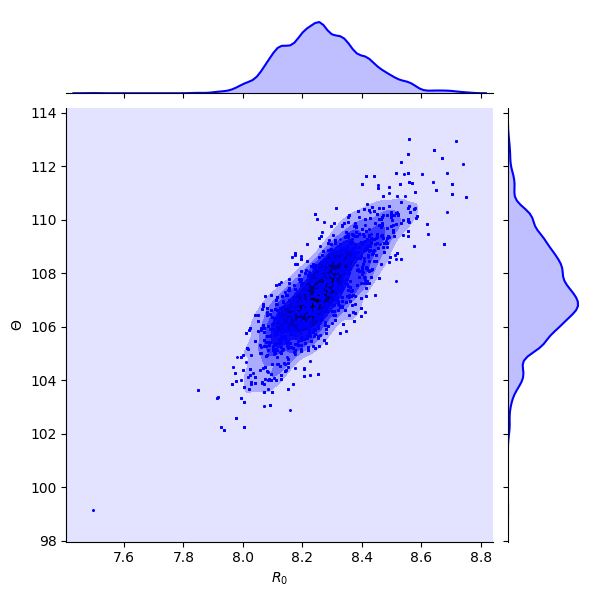
\includegraphics[width=0.9\textwidth]{../../sources/scripts/out.png}
\pagebreak
\subsection{Трехкомпонентное моделирование}
\subsubsection{Итеративное решение}
\subsubsection{Природная дисперсия}
% У заключения нет номера главы
\section*{Заключение}
\setmonofont[Mapping=tex-text]{CMU Typewriter Text}
\pagebreak
\bibliography{diploma.bib}
\bibliographystyle{ugost2008ls}
\end{document}
